\subsection{VGGT-Guided Densification}
\label{sec:depth_densify}

Silhouettes alone miss concave regions and fine structures. We densify the Visual Hull point cloud with \textbf{VGGT-Depth}: from a pre-trained VGGT backbone~\cite{Wang25_VGGT}, a depth prior adaptation branch with cross-attention over multi-view tokens and a lightweight fusion head predicts per-view depth and confidence. Unlike a frozen monocular depth network~\cite{Yang24_DepthAnythingV2}, the adaptation branch is conditioned on multi-view tokens (Figure~\ref{fig:vggt_depth}).

\begin{figure}[ht]
\centering
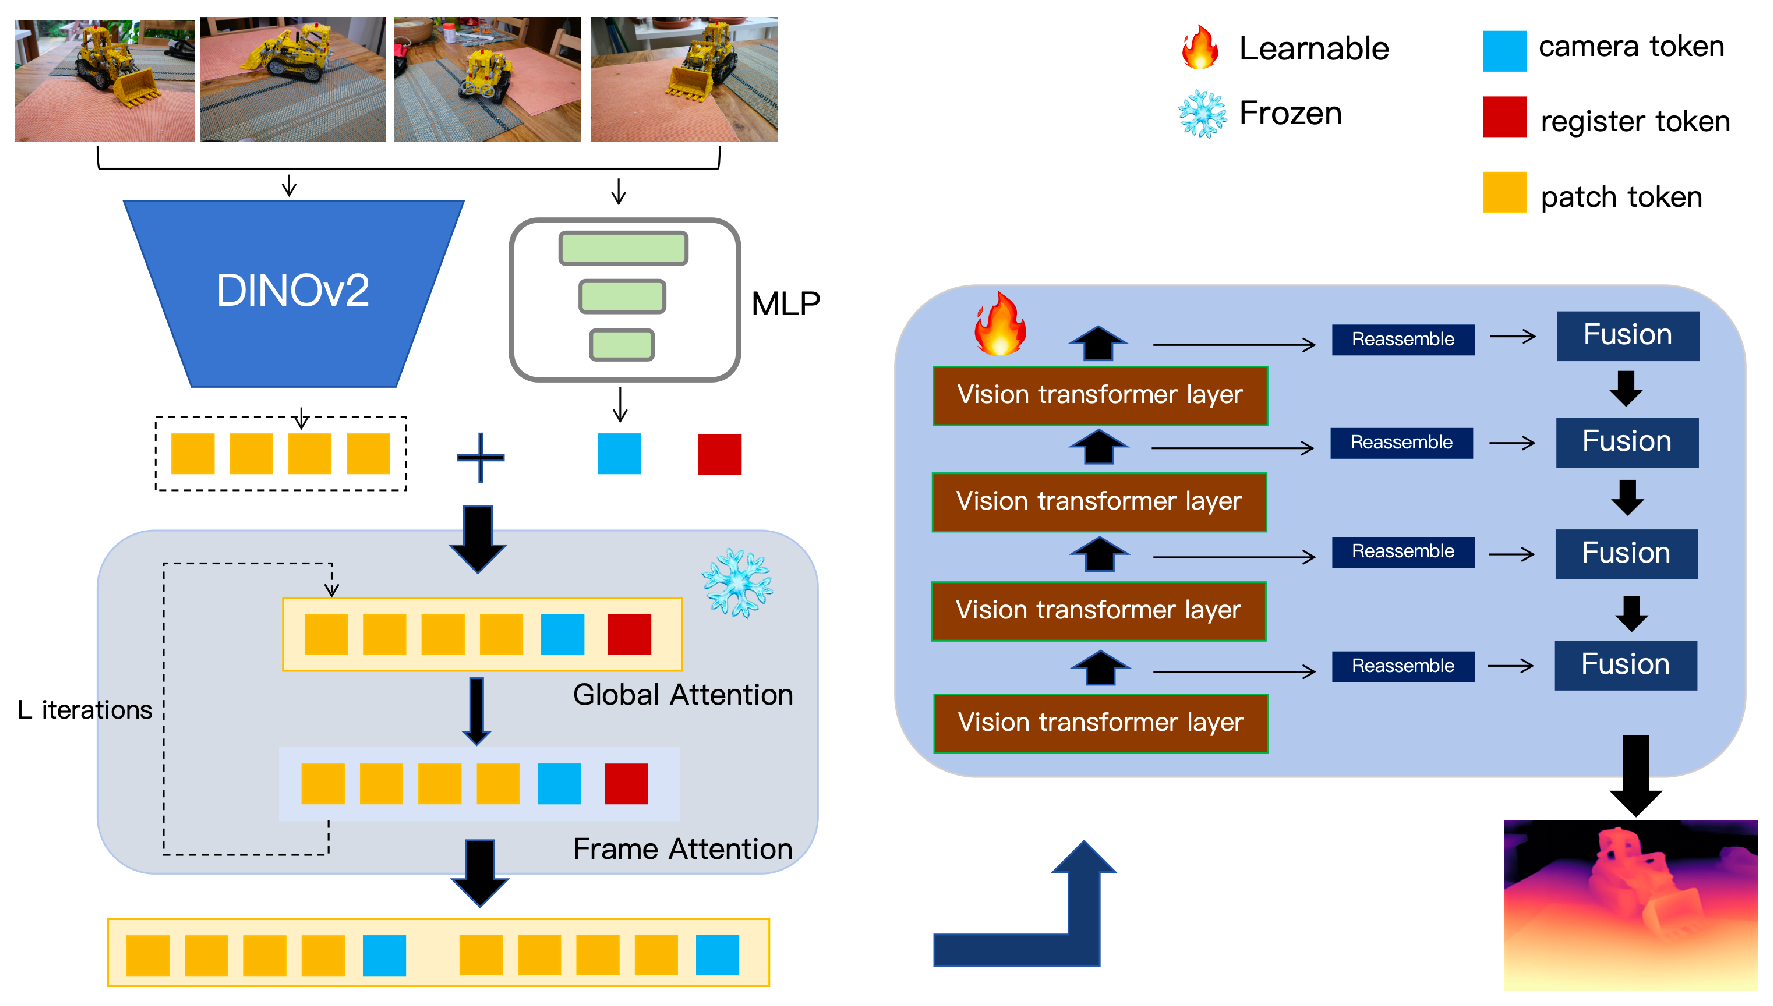
\includegraphics[width=0.90\textwidth]{figures/vggt_depth.pdf}
\caption{\label{fig:vggt_depth} VGGT-Depth prior used for depth-guided point cloud densification.}
\end{figure}

We use the Visual Hull AABB diagonal $L$ as the scene-scale reference. For each view, masked depth MAE against dataset ground-truth depth is used only to filter views and rays during densification (not at inference or when computing metrics); it is normalized by the 95th percentile over validation views to obtain $q_v$. Views with $q_v<0.4$ are discarded. If fewer than $0.8N$ views remain, densification is skipped and the Visual Hull point cloud is retained. Remaining views keep regions that pass VGGT-Depth confidence and depth consistency. With tolerance
\begin{equation}
\label{eq:delta_d}
\Delta(d)=\alpha d+\beta,\qquad
\alpha=0.01,\quad \beta=0.002L,
\end{equation}
we reject low-confidence or inconsistent observations before back-projection.

Point supplementation runs only along reliable rays. For each point, the top $K=3$ reliable views are selected; candidates are sampled around the predicted depth and back-projected. Here supplementation is applied offline to the Visual Hull point cloud before training. Complementary work injects epipolar depth priors into sparse-view Gaussian reconstruction~\cite{Zheng25_NexusGS}; we instead use adapted VGGT-Depth predictions for back-projection. Supplementary points are merged via two-stage voxel fusion and deduplication ($0.01L$ then $0.004L$).

\rev{Each densified point defines a Gaussian center, whose scale is initialized using the mean distance to its $k=8$ nearest neighbors. Color information from multiple views is combined using weights derived from depth consistency and VGGT confidence.} Opacity is set from cross-view consistency and clipped to $[0.2,0.8]$. Uneven supervision remains under sparse views; we address this with DVR (Sec.~\ref{sec:dvr}).

\rev{The initialization procedure separates the construction of the initial geometric support from the subsequent optimization of Gaussian attributes. Silhouette consistency first establishes the spatial envelope, whereas depth-based supplementation adds samples in regions that the initial representation may not describe adequately. These operations are completed before the Gaussian optimization stage. Consequently, the following regularization stage operates on an initialized representation that already incorporates the accepted geometric samples.}
